% Options for packages loaded elsewhere
\PassOptionsToPackage{unicode}{hyperref}
\PassOptionsToPackage{hyphens}{url}
%
\documentclass[
]{article}
\usepackage{amsmath,amssymb}
\usepackage{iftex}
\ifPDFTeX
  \usepackage[T1]{fontenc}
  \usepackage[utf8]{inputenc}
  \usepackage{textcomp} % provide euro and other symbols
\else % if luatex or xetex
  \usepackage{unicode-math} % this also loads fontspec
  \defaultfontfeatures{Scale=MatchLowercase}
  \defaultfontfeatures[\rmfamily]{Ligatures=TeX,Scale=1}
\fi
\usepackage{lmodern}
\ifPDFTeX\else
  % xetex/luatex font selection
\fi
% Use upquote if available, for straight quotes in verbatim environments
\IfFileExists{upquote.sty}{\usepackage{upquote}}{}
\IfFileExists{microtype.sty}{% use microtype if available
  \usepackage[]{microtype}
  \UseMicrotypeSet[protrusion]{basicmath} % disable protrusion for tt fonts
}{}
\makeatletter
\@ifundefined{KOMAClassName}{% if non-KOMA class
  \IfFileExists{parskip.sty}{%
    \usepackage{parskip}
  }{% else
    \setlength{\parindent}{0pt}
    \setlength{\parskip}{6pt plus 2pt minus 1pt}}
}{% if KOMA class
  \KOMAoptions{parskip=half}}
\makeatother
\usepackage{xcolor}
\usepackage[margin=1in]{geometry}
\usepackage{graphicx}
\makeatletter
\def\maxwidth{\ifdim\Gin@nat@width>\linewidth\linewidth\else\Gin@nat@width\fi}
\def\maxheight{\ifdim\Gin@nat@height>\textheight\textheight\else\Gin@nat@height\fi}
\makeatother
% Scale images if necessary, so that they will not overflow the page
% margins by default, and it is still possible to overwrite the defaults
% using explicit options in \includegraphics[width, height, ...]{}
\setkeys{Gin}{width=\maxwidth,height=\maxheight,keepaspectratio}
% Set default figure placement to htbp
\makeatletter
\def\fps@figure{htbp}
\makeatother
\setlength{\emergencystretch}{3em} % prevent overfull lines
\providecommand{\tightlist}{%
  \setlength{\itemsep}{0pt}\setlength{\parskip}{0pt}}
\setcounter{secnumdepth}{-\maxdimen} % remove section numbering
\ifLuaTeX
  \usepackage{selnolig}  % disable illegal ligatures
\fi
\usepackage{bookmark}
\IfFileExists{xurl.sty}{\usepackage{xurl}}{} % add URL line breaks if available
\urlstyle{same}
\hypersetup{
  pdftitle={Bike Share Analysis},
  pdfauthor={Jonathan Wong},
  hidelinks,
  pdfcreator={LaTeX via pandoc}}

\title{Bike Share Analysis}
\author{Jonathan Wong}
\date{2024-10-12}

\begin{document}
\maketitle

\subsubsection{Business Task:}\label{business-task}

\begin{enumerate}
\def\labelenumi{\arabic{enumi})}
\tightlist
\item
  To maximize the number of annual memberships for the company's future
  success
\item
  Compare casual riders vs.~annual members in their historical bike trip
  data
\item
  How can Cyclistic use digital media to convert casual riders into
  annual members
\end{enumerate}

\subsubsection{Resources Used:}\label{resources-used}

Amazon: \href{https://divvy-tripdata.s3.amazonaws.com/index.html}{Trip
Data}

\subsubsection{Documentation of Cleaning/Manipulating
Data:}\label{documentation-of-cleaningmanipulating-data}

\begin{figure}
\centering
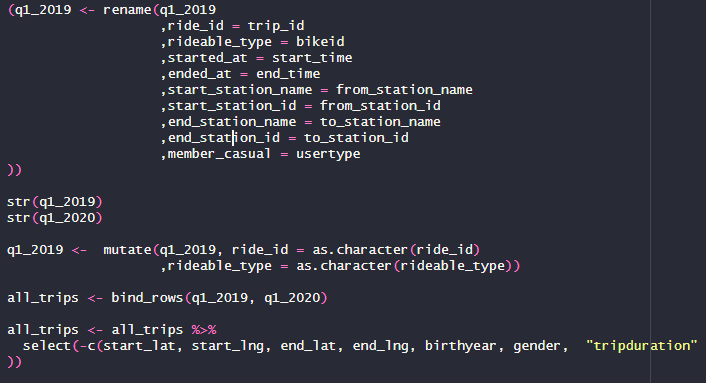
\includegraphics{Code_Image_1.png}
\caption{Combining Datasets}
\end{figure}

\begin{figure}
\centering
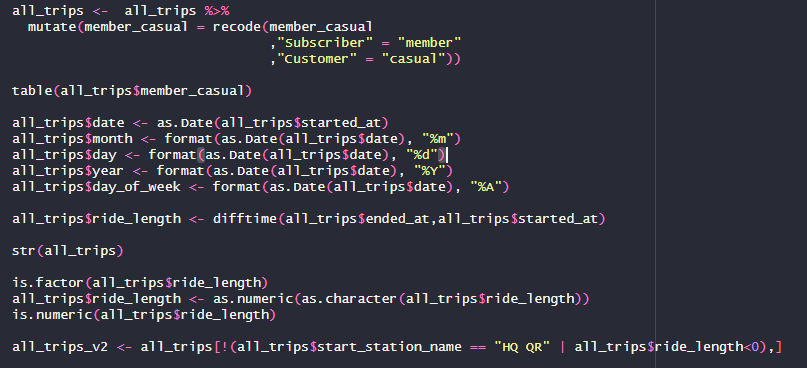
\includegraphics{Code_Image_2.png}
\caption{Data Clean Up}
\end{figure}

\subsubsection{Summary of Analysis:}\label{summary-of-analysis}

Based on my analysis, casual riders exhibited longer average, median,
and maximum ride duration compared to annual members. Notably, casual
ridership peaks on Thursdays and declines following the weekend. In
contrast, while annual member engagement remains consistently lower,
their average ride duration appears stable throughout the week.

In terms of overall ride volume, annual members significantly outnumber
casual riders. The patterns of engagement for these two groups are
inversely related; casual riders tend to peak during the weekends and
diminish during weekdays, whereas annual members demonstrate a
preference for weekday rides, often taking twice as many rides on those
days compared to weekends.

In summation, casual riders are taking longer rides with less overall
rides often peaking on the weekends. For annual members, they exhibit
shorter rides with more overall rides peaking on the weekdays. In terms
of the casual riders' behavior, they are inversely related with the
annual members.

\subsubsection{Visualizations/Key
Findings:}\label{visualizationskey-findings}

\paragraph{Average Ride Duration}\label{average-ride-duration}

\begin{verbatim}
##   user_type length_of_ride
## 1    casual      5372.7839
## 2    member       795.2523
\end{verbatim}

\paragraph{Median Ride Duration}\label{median-ride-duration}

\begin{verbatim}
##   user_type length_of_ride
## 1    casual           1393
## 2    member            508
\end{verbatim}

\paragraph{Maximum Ride Duration}\label{maximum-ride-duration}

\begin{verbatim}
##   user_type length_of_ride
## 1    casual       10632022
## 2    member        6096428
\end{verbatim}

\includegraphics{Bike_Share_Analysis_files/figure-latex/unnamed-chunk-8-1.pdf}
\includegraphics{Bike_Share_Analysis_files/figure-latex/unnamed-chunk-8-2.pdf}

\subsubsection{Recommendations:}\label{recommendations}

Based on my analysis, the data shows an inverse relationship in behavior
between casual riders and annual members. I propose the following three
recommendations:

\begin{enumerate}
\def\labelenumi{\arabic{enumi}.}
\item
  Conduct Comprehensive Surveys: We should implement surveys targeting
  both casual riders and annual members to gain deeper insights into
  their motivations and preferences. Understanding the perspectives of
  both groups will enable us to bridge the existing gap and enhance our
  conversion rates from casual to annual membership.
\item
  Incentivize Increased Ride Frequency: We recommend adjusting our
  pricing model to encourage casual riders to engage in more frequent,
  shorter rides rather than extended single rides. Additionally,
  streamlining the initial sign-up process for annual membership will
  enhance convenience and accessibility.
\item
  Promote Weekday Riding: We should market bike riding at Cyclistic as a
  viable option for weekday transportation, rather than solely as a
  weekend activity. This can be achieved by emphasizing the practicality
  of biking for commuting and other weekday errands, thereby broadening
  the appeal of our services to casual riders.
\end{enumerate}

By implementing these strategies, we can effectively align our offerings
with the needs of both casual and annual riders, ultimately driving
membership growth and engagement.

\end{document}
